
\documentclass[a4paper, twoside, svgnames]{report}

% package for splitting the page
\usepackage{paracol}

% Language and font encodings
\usepackage[english]{babel}
\usepackage[utf8x]{inputenc}
\usepackage[T1]{fontenc}
\usepackage{multirow}
% Sets page size and margins
\usepackage[a4paper,top=2cm,bottom=2cm,left=2cm,right=2cm,marginparwidth=1cm]{geometry}

% Useful packages
\usepackage{amsmath}
\usepackage{graphicx}
\usepackage[colorinlistoftodos]{todonotes}
\usepackage[colorlinks=true, allcolors=blue]{hyperref}
\usepackage{subfig}
\usepackage{graphicx}
\usepackage{comment}
\usepackage{float}
% For Summary
\usepackage{array}
\usepackage{adjustbox}
\newcolumntype{x}[1]{>{\centering\arraybackslash\hspace{0pt}}p{#1}}
\newcolumntype{M}[1]{>{\centering\arraybackslash}m{#1}}
\newcolumntype{C}[1]{>{\centering\let\newline\\\arraybackslash\hspace{0pt}}m{#1}}
\newcolumntype{P}[1]{>{\centering\arraybackslash}p{#1}}
\usepackage{caption}

\usepackage{multirow}
\renewcommand{\arraystretch}{1.2}





% Define custom colors if needed
\definecolor{myblue}{HTML}{41b7c8}
\definecolor{myred}{HTML}{fd1b14}
\definecolor{myyellow}{HTML}{fff535}
\definecolor{lightgreen}{RGB}{144,238,144}



\usepackage{fancyhdr}
\pagestyle{fancy}
\fancyhf{}
\rhead{15-11-2025\_16-06-12\_edison\_213522251444}
\lhead{
\includegraphics[width=3.5cm]{ logo_tight.png }}
\renewcommand{\footrulewidth}{1pt}


% For Figure
\usepackage{longtable, tabu}
\usepackage{pdflscape}


% For Radial Score
\usepackage{tikz}
\usepackage{calc}
\newlength{\outerradius}
\newlength{\innerradius}
\setlength{\outerradius}{0.5cm}
\setlength{\innerradius}{0.4cm}

\newcommand{\centered}[1]{\begin{tabular}{l} #1 \end{tabular}}

%Remark Box
\usepackage[svgnames]{xcolor}
\usepackage[framemethod=tikz]{mdframed}
\usetikzlibrary{shadows,shadings, calc}
\usepackage{calc}
\usepackage{tikz}
\usepackage{linegoal}

\usetikzlibrary{positioning}

%=====================================================================
% for radar chart
\newcommand{\D}{8} % number of dimensions (config option)
\newcommand{\U}{10} % number of scale units (config option)

\newdimen\R % maximal diagram radius (config option)
\R=2cm    % change the spider web radius
\newdimen\L % radius to put dimension labels (config option)
\L=2.8cm    % change the label radius

% for Joint Consistency Radar Chart
\newcommand{\J}{10} % number of dimensions (config option)
\newcommand{\JU}{10} % number of scale units (config option)
\newcommand{\JA}{360/\J} % calculated angle between dimension axes

\newcommand{\A}{360/\D} % calculated angle between dimension axes  
%=====================================================================
% for picture overlay
% pixel to cm
\pgfmathsetmacro{\pixelsToCm}{(3/4) * (2.54/72)} % 2.54 cm per inch, 72 points per inch, 1pt per 4/3 px
\newcommand{\pixelToCm}[2]{%
    \pgfmathsetmacro{#2}{#1*\pixelsToCm}%
}
% point to cm
\pgfmathsetmacro{\pointsToCm}{2.54/72} % 2.54 cm per inch, 72 points per inch, 1pt per 4/3 px
\newcommand{\pointToCm}[2]{%
    \pgfmathsetmacro{#2}{#1*\pointsToCm}%
}
% Define the line color globally
\colorlet{mylinecolor}{yellow} % Change 'blue' to the desired color
\colorlet{highlightcolor}{red}

%=====================================================================


\begin{document}

\setlength{\columnsep}{1cm}
\vspace*{0.5pt}
\vspace{-0.6cm}

\section*{\centering {\LARGE \textbf{\underline{ Edison Tan }}}}
\vspace{-0.1cm}

\columnratio{0.2099, 0.0001, 0.395, 0.395}
\begin{paracol}{4}
% left column
\switchcolumn[0]
\noindent % Ensures the following content starts at the left margin

\begin{minipage}[c]{\linewidth}
    
    % Measure the width and height of the image, in points
    \newlength{\imgwidth}
    \newlength{\imgheight}
    \settowidth{\imgwidth}{\includegraphics{ 00000.jpg }}
    \settoheight{\imgheight}{\includegraphics{ 00000.jpg }}
    % Width: \the\imgwidth    \   Height: \the\imgheight
    
    
    \pointToCm{\imgwidth}{\width}     
    \pointToCm{\imgheight}{\height}
    % Width: \width   \   Height: \height
    
    % Scale conversion
    \pixelToCm{191}{\headX}                      \pixelToCm{333}{\headY}
    \pixelToCm{228}{\leftshoulderX}      \pixelToCm{395}{\leftshoulderY}
    \pixelToCm{137}{\rightshoulderX}    \pixelToCm{411}{\rightshoulderY}
    \pixelToCm{295}{\leftelbowX}            \pixelToCm{378}{\leftelbowY}
    \pixelToCm{62}{\rightelbowX}          \pixelToCm{360}{\rightelbowY}
    \pixelToCm{380}{\leftwristX}            \pixelToCm{375}{\leftwristY}
    \pixelToCm{138}{\rightwristX}          \pixelToCm{354}{\rightwristY}
    \pixelToCm{235}{\lefthipX}                \pixelToCm{573}{\lefthipY}
    \pixelToCm{171}{\righthipX}              \pixelToCm{577}{\righthipY}
    \pixelToCm{257}{\leftkneeX}              \pixelToCm{681}{\leftkneeY}
    \pixelToCm{162}{\rightkneeX}            \pixelToCm{692}{\rightkneeY}
    \pixelToCm{288}{\leftankleX}            \pixelToCm{781}{\leftankleY}
    \pixelToCm{148}{\rightankleX}          \pixelToCm{799}{\rightankleY}
    \pixelToCm{182}{\midshoulderX}        \pixelToCm{403}{\midshoulderY}
    \pixelToCm{203}{\midhipX}                  \pixelToCm{575}{\midhipY}
    
    \centering
    \begin{minipage}{3.5cm}
        \centering
        \makebox[1.12\linewidth]{\textbf{Skeleton Joint}}
        \vspace{-0.3cm}
        
        \resizebox{0.8\linewidth}{!}{%
        \hspace{2cm}
        \centering                                    
            \begin{tikzpicture}[yscale=-1]      % yscale=-1 -> flip on x-axis
                \node[anchor=north west,inner sep=0] at (0.05,0)    {\includegraphics[width=360pt, height=640pt]{00000.jpg}};  % set the origin
                % \node[anchor=north west,inner sep=0] at (0,0)     {\includegraphics{00000.jpg}};  % set the origin
                
                \pointToCm{637.2}{\scaledHeight}
                
                % % plot the line (x-axis) and origin
                % \filldraw[cyan] (0,0) circle (3pt);
                % \draw[cyan] (0,0) -- ({0+\width}, 0);
    
                \coordinate (head) at (\headX, \headY);
                \coordinate (left_shoulder) at (\leftshoulderX, \leftshoulderY);
                \coordinate (right_shoulder) at (\rightshoulderX, \rightshoulderY);
                \coordinate (left_elbow) at (\leftelbowX, \leftelbowY);
                \coordinate (right_elbow) at (\rightelbowX, \rightelbowY);
                \coordinate (left_wrist) at (\leftwristX, \leftwristY);
                \coordinate (right_wrist) at (\rightwristX, \rightwristY);
                \coordinate (left_hip) at (\lefthipX, \lefthipY);
                \coordinate (right_hip) at (\righthipX, \righthipY);
                \coordinate (left_knee) at (\leftkneeX, \leftkneeY);
                \coordinate (right_knee) at (\rightkneeX, \rightkneeY);
                \coordinate (left_ankle) at (\leftankleX, \leftankleY);
                \coordinate (right_ankle) at (\rightankleX, \rightankleY);
                \coordinate (mid_shoulder) at (\midshoulderX, \midshoulderY);
                \coordinate (mid_hip) at (\midhipX, \midhipY);
                
                \coordinate (neck) at ($ (head) !0.6! (mid_shoulder) $);
                \coordinate (extended_neck) at ($ (neck) !-0.6! (mid_hip) $);
                \coordinate (extended_mid_shoulder) at ($ (mid_shoulder) !-0.6! (mid_hip) $);
                \coordinate (extended_hip) at ($ (neck) !2.3! (mid_hip) + (0.3,0) $);
    
                % Draw dots at coordinates (with label)
                \foreach \coord/\label in {
                    head/{},
                    left_shoulder/{J01},
                    right_shoulder/{J02},
                    left_elbow/{J03},
                    right_elbow/{J04},
                    left_wrist/{J05},
                    right_wrist/{J06},
                    left_hip/{},
                    right_hip/{},
                    left_knee/{J07},
                    right_knee/{J08},
                    left_ankle/{J09},
                    right_ankle/{J010},
                    mid_shoulder/{},
                    mid_hip/{}
                } {
                    \filldraw [yellow] (\coord) circle (3pt) node[anchor=west] {\label};    % scale here is in cm, node here is for the label
                }

                % Draw lines (human skeleton)
                \draw[mylinecolor] (head) -- (mid_shoulder);
                \draw[mylinecolor] (mid_shoulder) -- (left_shoulder);
                \draw[mylinecolor] (mid_shoulder) -- (right_shoulder);
                \draw[mylinecolor] (mid_shoulder) -- (mid_hip);
                \draw[mylinecolor] (right_shoulder) -- (right_elbow);
                \draw[mylinecolor] (right_elbow) -- (right_wrist);
                \draw[mylinecolor] (left_shoulder) -- (left_elbow);
                \draw[mylinecolor] (left_elbow) -- (left_wrist);
                \draw[mylinecolor] (mid_hip) -- (right_hip);
                \draw[mylinecolor] (right_hip) -- (right_knee);
                \draw[mylinecolor] (right_knee) -- (right_ankle);
                \draw[mylinecolor] (mid_hip) -- (left_hip);
                \draw[mylinecolor] (left_hip) -- (left_knee);
                \draw[mylinecolor] (left_knee) -- (left_ankle);
                
                % Highlight the specify coordinate                    
                \draw[green, line width=0.45cm, opacity=0.3] (extended_mid_shoulder) -- (extended_hip);
                \draw[highlightcolor, line width=0.45cm, opacity=0.3] (right_shoulder) -- (\rightshoulderX, 0.75\scaledHeight);
                \draw[highlightcolor, line width=0.45cm, opacity=0.3] (left_shoulder) -- (\leftshoulderX, 0.75\scaledHeight);
            \end{tikzpicture}                
        }%
    \end{minipage}%
    
    
    \vspace{1cm}
    \begin{minipage}{4cm}
        \centering
        \textbf{Hand Release}
        \vspace{0.2cm}
        
        % Enlarged Display
        \adjincludegraphics[height=4cm, width=3.5cm, trim={0 0 {0.5\width} 0},clip]{ 00069.jpg } % Left Half
        
    \end{minipage}
\end{minipage}

\switchcolumn[2]
\begin{minipage}[c]{\linewidth}

    \begin{minipage}{\linewidth}
        \hspace{0.05cm}
        \resizebox{\linewidth}{!}{
        
\begin{tikzpicture}[scale=1]
            \path (0:0cm) coordinate (O); % define coordinate for origin                    

            % draw the spiderweb
            \foreach \X in {1,...,\D}{
            \draw (\X*\A:0) -- (\X*\A:\R);
            }
        
            \foreach \Y in {0,...,\U}{
            \foreach \X in {1,...,\D}{
                \path (\X*\A:\Y*\R/\U) coordinate (D\X-\Y);
                \fill (D\X-\Y) circle (1pt);
            }
            \draw [opacity=0.3] (0:\Y*\R/\U) \foreach \X in {1,...,\D}{
                -- (\X*\A:\Y*\R/\U)
            } -- cycle;
            }
        
            % define labels for each dimension axis (names config option)
            %\path (1*\A:\L) node (L1) {Consistency};
            %\path (2*\A:\L) node (L2) {Grouping};
            %\path (3*\A:\L) node (L3) {Aiming};
            %\path (4*\A:\L) node (L4) {Strength};     


            %D1 - Consistency
            %D2 - Grouping
            %D3 - Aiming
            %D4 - Strength
            %D5 - Bow Balance
            %D6 - Bow Stability
            %D7 - Anchor
            %D8 - DFL
            \path (1*\A:\L) node (L1) [align=center]{\footnotesize Consistency\\ \footnotesize 91.26\%};
            \path (2*\A:\L) node (L2) [align=center]{\footnotesize Grouping\\ \footnotesize 93.21\%};
            \path (3*\A:\L) node (L3) [align=center]{\footnotesize Aiming\\ \footnotesize 58.97\%};
            \path (4*\A:\L) node (L4) [align=center]{\footnotesize Strength\\ \footnotesize 75.79\%};
            \path (5*\A:\L) node (L5) [align=center]{\footnotesize Bow Balance\\ \footnotesize 96.85\%};
            \path (6*\A:\L) node (L6) [align=center]{\footnotesize Bow Stability\\ \footnotesize 88.87\%};
            \path (7*\A:\L) node (L7) [align=center]{\footnotesize Anchor\\ \footnotesize 90.01\%};
            \path (8*\A:\L) node (L8) [align=center]{\footnotesize DFL\\ \footnotesize 80.41\%};
            
            
            \draw [fill=red, color=red,line width=1.5pt,opacity=0.5]
            (D1-8.726) --
            (D2-9.181) --
            (D3-4.301) --
            (D4-7.075) --
            (D5-9.685) --
            (D6-8.887) --
            (D7-9.001) --
            (D8-8.041) -- cycle;
        
        \end{tikzpicture}            
    }
    \end{minipage}%
    
    \vspace{0.5cm}
    
    
    \begin{minipage}{\linewidth}
        \resizebox{1.05\linewidth}{!}{%   
        \hspace{0.1cm}
        \centering
        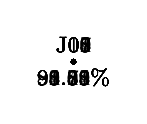
\begin{tikzpicture}[scale=1]
            \path (0:0cm) coordinate (O); % define coordinate for origin
        
              % draw the spiderweb
              \foreach \X in {1,...,\J}{
                \draw (\X*\JA:0) -- (\X*\JA:\R);
              }
        
              \foreach \Y in {0,...,\JU}{
                \foreach \X in {1,...,\J}{
                  \path (\X*\JA:\Y*\R/\JU) coordinate (D\X-\Y);
                  \fill (D\X-\Y) circle (1pt);
                }
                \draw [opacity=0.3] (0:\Y*\R/\JU) \foreach \X in {1,...,\J}{
                    -- (\X*\JA:\Y*\R/\JU)
                } -- cycle;
              }
            
        
            % define labels for each dimension axis (names config option)
            \path (1*\JA:\L) node (L1) [align=center]{\footnotesize J02\\ \footnotesize 94.45\%};
            \path (2*\JA:\L) node (L2) [align=center]{\footnotesize J01\\ \footnotesize 91.26\%};
            \path (3*\JA:\L) node (L3) [align=center]{\footnotesize J10\\ \footnotesize 91.33\%};
            \path (4*\JA:\L) node (L4) [align=center]{\footnotesize J09\\ \footnotesize 98.88\%};
            \path (5*\JA:\L) node (L5) [align=center]{\footnotesize J08\\ \footnotesize 95.84\%};
            \path (6*\JA:\L) node (L6) [align=center]{\footnotesize J07\\ \footnotesize 92.69\%};
            \path (7*\JA:\L) node (L7) [align=center]{\footnotesize J06\\ \footnotesize 86.82\%};
            \path (8*\JA:\L) node (L8) [align=center]{\footnotesize J05\\ \footnotesize 93.75\%};
            \path (9*\JA:\L) node (L9) [align=center]{\footnotesize J04\\ \footnotesize 89.71\%};
            \path (10*\JA:\L) node (L10) [align=center]{\footnotesize J03\\ \footnotesize 93.09\%};
            
            %D1 = J02
            %D2 = J01
            %D3 = J10
            %D4 = J09
            %D5 = J08
            %D6 = J07
            %D7 = J06
            %D8 = J05
            %D9 = J04
            %D10 = J03
            
            \draw [fill=green, color=green,line width=1.5pt,opacity=0.5]
            (D1-9.126) --
            (D2-9.445) --
            (D3-9.309) --
            (D4-8.971) --
            (D5-9.375) --
            (D6-8.682) --
            (D7-9.269) --
            (D8-9.584) --
            (D9-9.888) --
            (D10-9.133) -- cycle;
        
        \end{tikzpicture}
    }
    \end{minipage}%
    
\end{minipage}

\switchcolumn[3]
\begin{minipage}[c]{\linewidth}
    \centering
    \framebox[\linewidth][r]{
        \begin{minipage}[t][5cm][t]{\linewidth}
            \centering
            \vspace{0.1cm}
            \scriptsize
            \begin{itemize}
                \setlength{\itemsep}{0pt}
                % Add items here: \item <Text>
                \item Sample Item.
            \end{itemize}
        \end{minipage}
    }
    
    \vspace{0.35cm}
    
    % score table    
    \centering
    \begin{minipage}{\linewidth}                  
        \begin{center}
            \textbf{Score}
            \vspace{-0.1cm}

            \textbf{\textcolor{LightCoral}{\scriptsize 9}} -                    \textbf{\textcolor{SkyBlue}{\scriptsize 10}} -                    \textbf{\textcolor{MediumSpringGreen}{\scriptsize 10}} -                    \textbf{\textcolor{Turquoise}{\scriptsize 9}} -                    \textbf{\textcolor{Orchid}{\scriptsize 8}} -\\
            \vspace{-0.2cm}
            \textbf{\textcolor{LightSeaGreen}{\scriptsize 10}} -                    \textbf{\textcolor{SandyBrown}{\scriptsize 9}} -                    \textbf{\textcolor{CornflowerBlue}{\scriptsize 9}} -                    \textbf{\textcolor{Silver}{\scriptsize 10}} -                    \textbf{\textcolor{LightSlateGray}{\scriptsize 10}}  
        \end{center}
    \end{minipage}%    
    \vspace{0.1cm}
    
    
    % target
    \centering
    \begin{minipage}{0.9\linewidth}
        
        \centering
        \resizebox{0.7\linewidth}{!}{%
        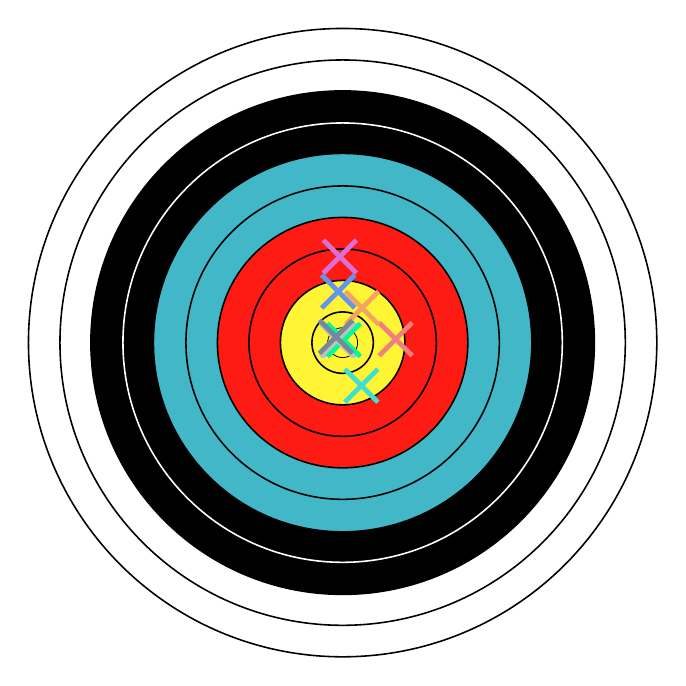
\begin{tikzpicture}
        % Zones
        \draw[fill=white,draw=black,line width=0.2mm] (0,0) circle (39.9mm);
        \draw[fill=white,draw=black,line width=0.2mm] (0,0) circle (35.9mm);
        \draw[fill=black] (0,0) circle (32mm);
        \draw[fill=black,draw=white,line width=0.2mm] (0,0) circle (27.9mm);
        \draw[fill=myblue] (0,0) circle (24mm);
        \draw[fill=myblue,draw=black,line width=0.2mm] (0,0) circle (19.9mm);
        \draw[fill=myred,draw=black,line width=0.2mm] (0,0) circle (15.9mm);
        \draw[fill=myred,draw=black,line width=0.2mm] (0,0) circle (11.9mm);
        \draw[fill=myyellow,draw=black,line width=0.2mm] (0,0) circle (7.9mm);
        \draw[fill=myyellow,draw=black,line width=0.2mm] (0,0) circle (3.9mm);
        \draw[fill=myyellow,draw=black,line width=0.1mm] (0,0) circle (1.9mm);
        \draw[black,line width=0.1mm] (-0.2mm,0) -- (0.2mm,0);
        \draw[black,line width=0.1mm] (0,-0.2mm) -- (0,0.2mm);
        
        
        % Get the color for this index from the lookup table
        \definecolor{crosscolor}{named}{ LightCoral }

        % Draw the cross using the color from the lookup table
        \draw[crosscolor, line width=0.6mm] 
            (46.74mm-40mm-2.1mm,-39.56mm+40mm-2.1mm) -- (46.74mm-40mm+2.1mm,-39.56mm+40mm+2.1mm)
            (46.74mm-40mm+2.1mm,-39.56mm+40mm-2.1mm) -- (46.74mm-40mm-2.1mm,-39.56mm+40mm+2.1mm);
                % Get the color for this index from the lookup table
        \definecolor{crosscolor}{named}{ SkyBlue }

        % Draw the cross using the color from the lookup table
        \draw[crosscolor, line width=0.6mm] 
            (39.58mm-40mm-2.1mm,-39.65mm+40mm-2.1mm) -- (39.58mm-40mm+2.1mm,-39.65mm+40mm+2.1mm)
            (39.58mm-40mm+2.1mm,-39.65mm+40mm-2.1mm) -- (39.58mm-40mm-2.1mm,-39.65mm+40mm+2.1mm);
                % Get the color for this index from the lookup table
        \definecolor{crosscolor}{named}{ MediumSpringGreen }

        % Draw the cross using the color from the lookup table
        \draw[crosscolor, line width=0.6mm] 
            (40.15mm-40mm-2.1mm,-39.66mm+40mm-2.1mm) -- (40.15mm-40mm+2.1mm,-39.66mm+40mm+2.1mm)
            (40.15mm-40mm+2.1mm,-39.66mm+40mm-2.1mm) -- (40.15mm-40mm-2.1mm,-39.66mm+40mm+2.1mm);
                % Get the color for this index from the lookup table
        \definecolor{crosscolor}{named}{ Turquoise }

        % Draw the cross using the color from the lookup table
        \draw[crosscolor, line width=0.6mm] 
            (42.38mm-40mm-2.1mm,-45.45615242270663mm+40mm-2.1mm) -- (42.38mm-40mm+2.1mm,-45.45615242270663mm+40mm+2.1mm)
            (42.38mm-40mm+2.1mm,-45.45615242270663mm+40mm-2.1mm) -- (42.38mm-40mm-2.1mm,-45.45615242270663mm+40mm+2.1mm);
                % Get the color for this index from the lookup table
        \definecolor{crosscolor}{named}{ Orchid }

        % Draw the cross using the color from the lookup table
        \draw[crosscolor, line width=0.6mm] 
            (39.65mm-40mm-2.1mm,-29.08mm+40mm-2.1mm) -- (39.65mm-40mm+2.1mm,-29.08mm+40mm+2.1mm)
            (39.65mm-40mm+2.1mm,-29.08mm+40mm-2.1mm) -- (39.65mm-40mm-2.1mm,-29.08mm+40mm+2.1mm);
                % Get the color for this index from the lookup table
        \definecolor{crosscolor}{named}{ LightSeaGreen }

        % Draw the cross using the color from the lookup table
        \draw[crosscolor, line width=0.6mm] 
            (39.17mm-40mm-2.1mm,-39.26mm+40mm-2.1mm) -- (39.17mm-40mm+2.1mm,-39.26mm+40mm+2.1mm)
            (39.17mm-40mm+2.1mm,-39.26mm+40mm-2.1mm) -- (39.17mm-40mm-2.1mm,-39.26mm+40mm+2.1mm);
                % Get the color for this index from the lookup table
        \definecolor{crosscolor}{named}{ SandyBrown }

        % Draw the cross using the color from the lookup table
        \draw[crosscolor, line width=0.6mm] 
            (42.47mm-40mm-2.1mm,-35.59384757729337mm+40mm-2.1mm) -- (42.47mm-40mm+2.1mm,-35.59384757729337mm+40mm+2.1mm)
            (42.47mm-40mm+2.1mm,-35.59384757729337mm+40mm-2.1mm) -- (42.47mm-40mm-2.1mm,-35.59384757729337mm+40mm+2.1mm);
                % Get the color for this index from the lookup table
        \definecolor{crosscolor}{named}{ CornflowerBlue }

        % Draw the cross using the color from the lookup table
        \draw[crosscolor, line width=0.6mm] 
            (39.44mm-40mm-2.1mm,-33.5mm+40mm-2.1mm) -- (39.44mm-40mm+2.1mm,-33.5mm+40mm+2.1mm)
            (39.44mm-40mm+2.1mm,-33.5mm+40mm-2.1mm) -- (39.44mm-40mm-2.1mm,-33.5mm+40mm+2.1mm);
                % Get the color for this index from the lookup table
        \definecolor{crosscolor}{named}{ Silver }

        % Draw the cross using the color from the lookup table
        \draw[crosscolor, line width=0.6mm] 
            (39.3mm-40mm-2.1mm,-39.7mm+40mm-2.1mm) -- (39.3mm-40mm+2.1mm,-39.7mm+40mm+2.1mm)
            (39.3mm-40mm+2.1mm,-39.7mm+40mm-2.1mm) -- (39.3mm-40mm-2.1mm,-39.7mm+40mm+2.1mm);
                % Get the color for this index from the lookup table
        \definecolor{crosscolor}{named}{ LightSlateGray }

        % Draw the cross using the color from the lookup table
        \draw[crosscolor, line width=0.6mm] 
            (39.16mm-40mm-2.1mm,-39.27mm+40mm-2.1mm) -- (39.16mm-40mm+2.1mm,-39.27mm+40mm+2.1mm)
            (39.16mm-40mm+2.1mm,-39.27mm+40mm-2.1mm) -- (39.16mm-40mm-2.1mm,-39.27mm+40mm+2.1mm);
            
        \end{tikzpicture}            
        }% 
    \end{minipage}%

\end{minipage}
\end{paracol}

\begin{center}
    \captionsetup{singlelinecheck = false, justification=justified, labelformat = empty, skip=1pt}
    
    \begin{figure*}[!h]
        \centering
        \resizebox{1\textwidth}{!}{
        \begin{tabular}{C{0.15\linewidth}C{0.15\linewidth}C{0.15\linewidth}C{0.15\linewidth}C{0.15\linewidth}}
            % First row of images
            %J01
            \begin{minipage}{\linewidth}\centering
                \includegraphics[width=\linewidth]{ processed_jointset_0.png }
                \caption{\scriptsize } % <---- remarks/captions go here
            \end{minipage} &
            
            %J02
            \begin{minipage}{\linewidth}\centering
                \includegraphics[width=\linewidth]{ processed_jointset_1.png }
                \caption{\scriptsize } % <---- remarks/captions go here
            \end{minipage} &
            
            %J03
            \begin{minipage}{\linewidth}\centering
                \includegraphics[width=\linewidth]{ processed_jointset_2.png }
                \caption{\scriptsize } % <---- remarks/captions go here
            \end{minipage} &
            
            %J04
            \begin{minipage}{\linewidth}\centering
                \includegraphics[width=\linewidth]{ processed_jointset_3.png }
                \caption{\scriptsize } % <---- remarks/captions go here
            \end{minipage} &
            
            %J05
            \begin{minipage}{\linewidth}\centering
                \includegraphics[width=\linewidth]{ processed_jointset_4.png }
                \caption{\scriptsize } % <---- remarks/captions go here
            \end{minipage} \\
            
            \\[-5pt]
            
            % Second row of images
            %J06
            \begin{minipage}{\linewidth}\centering
                \includegraphics[width=\linewidth]{ processed_jointset_5.png } 
                \caption{\scriptsize } % <---- remarks/captions go here
            \end{minipage} &
            
            %J07
            \begin{minipage}{\linewidth}\centering
                \includegraphics[width=\linewidth]{ processed_jointset_6.png } 
                \caption{\scriptsize } % <---- remarks/captions go here
            \end{minipage} &
            
            %J08
            \begin{minipage}{\linewidth}\centering
                \includegraphics[width=\linewidth]{ processed_jointset_7.png }
                \caption{\scriptsize } % <---- remarks/captions go here
            \end{minipage} &
            
            %J09
            \begin{minipage}{\linewidth}\centering
                \includegraphics[width=\linewidth]{ processed_jointset_8.png } 
                \caption{\scriptsize } % <---- remarks/captions go here
            \end{minipage} &
            
            %J10
            \begin{minipage}{\linewidth}\centering
                \includegraphics[width=\linewidth]{ processed_jointset_9.png }
                \caption{\scriptsize } % <---- remarks/captions go here
            \end{minipage} \\
        \end{tabular}}
    \end{figure*}
\end{center}

    
\end{document}
